\documentclass[11pt,letterpaper]{article}
\usepackage[margin=0.85in,headheight=14pt]{geometry}
\usepackage{amsmath,amssymb}
\usepackage{enumitem}
\usepackage{fancyhdr}
\usepackage{lmodern}
\usepackage[T1]{fontenc}
\usepackage[dvipsnames]{xcolor}
\usepackage[most]{tcolorbox}
\usepackage{pgfplots}
\usepgfplotslibrary{groupplots,fillbetween}
\usetikzlibrary{arrows.meta,positioning,shapes.geometric,calc,decorations.markings}
\pgfplotsset{
  compat=1.18,
  every axis/.append style={grid=major, grid style={gray!25}, tick label style={font=\footnotesize},
    label style={font=\small}, title style={font=\small}, legend style={font=\scriptsize}},
}
\definecolor{cA}{HTML}{1F77B4}
\definecolor{cB}{HTML}{FF7F0E}
\definecolor{cC}{HTML}{2CA02C}
\definecolor{cD}{HTML}{D62728}
\definecolor{cE}{HTML}{9467BD}

\pagestyle{fancy}
\fancyhf{}
\lhead{SYDE 556/750 \qquad Practice Test 3B}
\rhead{Solutions \& marking guide}
\cfoot{\thepage}
\renewcommand{\headrulewidth}{0pt}

\setlength{\parindent}{0pt}
\setlength{\parskip}{4pt}

\newcommand{\tref}{\tau_{\mathrm{ref}}}
\newcommand{\trc}{\tau_{RC}}
\newcommand{\tin}{\tau_{\mathrm{in}}}
\newcommand{\ans}[1]{\par\vspace{4pt}{\bfseries #1}\quad}

\newtcolorbox{marking}{colback=blue!3,colframe=blue!40!black,boxrule=0.4pt,left=4pt,right=4pt,top=2pt,bottom=2pt,arc=1pt,fonttitle=\bfseries\small,title=Marking}
\newtcolorbox{trap}{colback=red!4,colframe=red!50!black,boxrule=0.4pt,left=4pt,right=4pt,top=2pt,bottom=2pt,arc=1pt,fonttitle=\bfseries\small,title=Where marks are usually lost}

\tikzset{
  declare function={lif(\z,\tr,\tc,\Jm) = (\z > 0) * 1/(\tr - \tc*ln(1 - 1/(1 + (\Jm-1)*max(\z,1e-6))));},
}

\begin{document}

\begin{center}
{\Large\bfseries Practice Test 3B: Nengo \& Simple Dynamics --- Solutions}\\[2pt]
Total: 20 marks plus 2 bonus. Simulation data: \texttt{pn3\_data/make\_data\_3b.py} (Nengo 4).
\end{center}

%=====================================================================
\section*{Question 1 \hfill (4)}

\ans{(a) [2]}
A neuron only ``sees'' the part of $\mathbf x$ along its encoder, $\langle e, \mathbf x\rangle$. Nengo intercepts and max rates are in normalized units, so the neuron sees $\langle e, \mathbf x\rangle / R$, with $R = 2$.
\begin{itemize}[leftmargin=1.2em]
\item \textbf{Along $(0, s)$:} $\langle e, \mathbf x\rangle = s$. The neuron starts firing at $s/R = -0.5$, i.e.\ at $s = -1$, and rises with the LIF shape to $150$ Hz at $s = R = 2$. Below $s = -1$ it is silent.
\item \textbf{Along $(s, 0)$:} $\langle e, \mathbf x\rangle = 0$ for every $s$, so the current never changes. The rate is a \textbf{flat line} at the value of the first curve at $s = 0$. That value is positive because the intercept is negative: about $74$ Hz with $\tref = 2$ ms and $\trc = 20$ ms (any value between $0$ and $150$ earns the mark).
\end{itemize}
\begin{center}
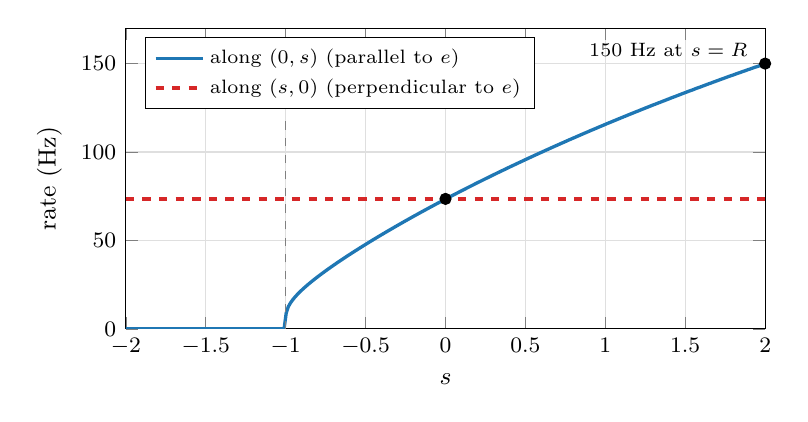
\begin{tikzpicture}
\begin{axis}[width=0.8\textwidth, height=5.4cm, xmin=-2, xmax=2, ymin=0, ymax=170,
  xlabel={$s$}, ylabel={rate (Hz)}, legend pos=north west, legend cell align=left]
  \addplot[cA, very thick, domain=-2:2, samples=300] {lif((x/2+0.5)/1.5, 0.002, 0.02, 4.805)};
  \addplot[cD, very thick, dashed, domain=-2:2, samples=2] {73.5};
  \legend{{along $(0, s)$ (parallel to $e$)}, {along $(s, 0)$ (perpendicular to $e$)}}
  \draw[gray, dashed] (axis cs:-1,0) -- (axis cs:-1,120) node[above, font=\scriptsize, black] {$s = -1 = -0.5R$};
  \addplot[only marks, mark=*, black] coordinates {(2,150) (0,73.5)};
  \node[font=\scriptsize, anchor=east] at (axis cs:1.95,158) {$150$ Hz at $s = R$};
\end{axis}
\end{tikzpicture}
\end{center}
\begin{marking}
0.5: parallel curve is zero below $s = -1$. \ 0.5: it rises to $150$ Hz at $s = 2$ (not at $s = 1$). \ 1: perpendicular line is constant and nonzero, matching the parallel curve at $s = 0$.
\end{marking}
\begin{trap}
Putting the threshold at $s = -0.5$ (forgetting the radius), or drawing the perpendicular case as a second tuning curve. Movement perpendicular to $e$ is invisible to this neuron.
\end{trap}

\ans{(b) [2]}
The probe synapse only filters the \emph{recorded} value. It is a measurement choice, so it does \textbf{not} change what the ensemble represents or anything downstream. Each probe is a low-pass filter on the decoded spikes, applied to a $2$ Hz sine ($\omega = 4\pi$ rad/s):
\begin{itemize}[leftmargin=1.2em]
\item \texttt{0.001}: almost unfiltered, so the trace is \textbf{very noisy} (each spike shows up as a sharp jump) but has no visible lag.
\item \texttt{0.01}: a little smoothing and a small lag. This gives the cleanest picture of the represented value.
\item \texttt{0.1}: smooth, but \textbf{attenuated and delayed}. The gain is $1/\sqrt{1 + (\omega\tau)^2} = 1/\sqrt{1 + (0.4\pi)^2} \approx 0.62$ and the lag is $\arctan(0.4\pi)/\omega \approx 72$ ms.
\end{itemize}
\begin{center}
\begin{tikzpicture}
\begin{axis}[width=0.95\textwidth, height=5.6cm, xmin=0, xmax=1, ymin=-1.8, ymax=1.8,
  xlabel={$t$ (s)}, ylabel={probed $\hat x$}, legend style={at={(0.5,1.02)}, anchor=south}, legend cell align=left, legend columns=4]
  \addplot[cB, thin, opacity=0.55] table[x=t, y=p1] {pn3_data/q1b_probes.dat};
  \addplot[cA, very thick] table[x=t, y=p10] {pn3_data/q1b_probes.dat};
  \addplot[cD, very thick] table[x=t, y=p100] {pn3_data/q1b_probes.dat};
  \addplot[black, dashed, thick] table[x=t, y=x] {pn3_data/q1b_probes.dat};
  \legend{{\texttt{synapse=0.001}}, {\texttt{synapse=0.01}}, {\texttt{synapse=0.1}}, {$x(t)$}}
\end{axis}
\end{tikzpicture}
\end{center}
\begin{marking}
0.5: small synapse is the noisiest. \ 0.5: large synapse is smoother, \emph{smaller} and \emph{later}. \ 1: the probe synapse does not change the representation (it only filters what is recorded).
\end{marking}

%=====================================================================
\section*{Question 2 \hfill (4)}

\ans{(a) [2]}
\begin{itemize}[leftmargin=1.2em]
\item $x$: the value the population represents (decoded from its activity).
\item $g(u)$: what the input connection computes. It is decoded from the input population with function decoders and arrives through the synapse.
\item $f(x)$: what the recurrent connection computes. The population decodes $f(x)$ from its own activity and feeds it back to itself.
\item $\tau$: the synaptic time constant. It sets the timescale, because nothing reaches the population faster than the synapse allows.
\item $-x$: this comes from the \textbf{synapse}, not from any connection. Everything arriving at the population is filtered: $x = h * (g(u) + f(x))$. In the Laplace domain this is $X = (G + F)/(1 + s\tau)$, so $\tau sX = G + F - X$, i.e.\ $\tau\dot x = g(u) + f(x) - x$. The $-x$ is the synapse's own decay.
\end{itemize}
\textbf{No recurrence} ($f = 0$): $\tau\dot x = g(u) - x$, so $x$ is just $g(u)$ low-pass filtered by the synapse. It follows the input with time constant $\tau$ and forgets it within a few $\tau$ once the input goes away.
\begin{marking}
0.25 each for $x$, $g$, $f$, $\tau$ (1). \ 0.5: $-x$ comes from the synapse filter. \ 0.5: without recurrence $x$ is the synapse low-pass of $g(u)$ and decays to zero after the input stops.
\end{marking}

\ans{(b) [2]}
Here $A = -1/0.5 = -2$ and $B = 1/0.5 = 2$. Match $\tau\dot x = (A'-1)x + B'u$ to $\tau\dot x = \tau A x + \tau B u$:
\[
A' = \tau A + 1 = 0.05(-2) + 1 = \mathbf{0.9}, \qquad B' = \tau B = 0.05(2) = \mathbf{0.1}.
\]
\textbf{Network:} an input node $u$ connects to the population $x$ with \texttt{transform=0.1, synapse=0.05}, and $x$ connects to itself with \texttt{transform=0.9, synapse=0.05}. The step response has time constant $\mathbf{0.5}$ \textbf{s}, which is $\tau/(1 - A') = 0.05/0.1$: the network is 10 times slower than the synapse. It settles at $B'/(1 - A') = 1$ for a unit step.
\begin{center}
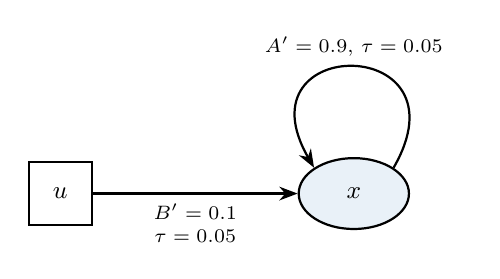
\begin{tikzpicture}[font=\small, node distance=1.4cm,
  pop/.style={draw, thick, ellipse, minimum width=1.4cm, minimum height=0.9cm, fill=cA!10}]
  \node[draw, thick, minimum size=0.8cm] (u) {$u$};
  \node[pop, right=2.6cm of u] (x) {$x$};
  \draw[-{Stealth}, thick] (u) -- node[below, font=\scriptsize, align=center] {$B' = 0.1$\\$\tau = 0.05$} (x);
  \draw[-{Stealth}, thick] (x.north east) to[out=60, in=120, looseness=5] node[above, font=\scriptsize] {$A' = 0.9$, $\tau = 0.05$} (x.north west);
\end{tikzpicture}
\hspace{0.3cm}
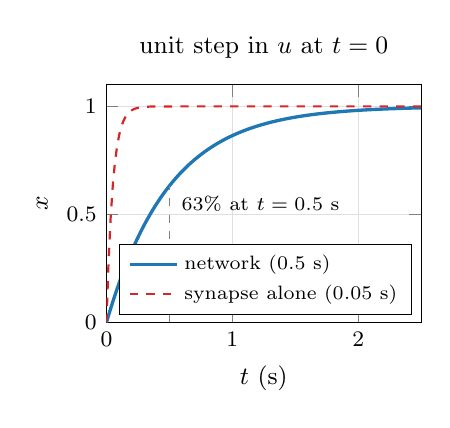
\begin{tikzpicture}[baseline=(current bounding box.center)]
\begin{axis}[width=0.46\textwidth, height=4.6cm, xmin=0, xmax=2.5, ymin=0, ymax=1.1,
  xlabel={$t$ (s)}, ylabel={$x$}, legend pos=south east, legend cell align=left, title={unit step in $u$ at $t = 0$}]
  \addplot[cA, very thick, domain=0:2.5, samples=150] {1 - exp(-x/0.5)};
  \addplot[cD, thick, dashed, domain=0:2.5, samples=150] {1 - exp(-x/0.05)};
  \legend{network ($0.5$ s), synapse alone ($0.05$ s)}
  \draw[gray, dashed] (axis cs:0.5,0) -- (axis cs:0.5,0.632);
  \node[font=\scriptsize, anchor=west] at (axis cs:0.52,0.55) {$63\%$ at $t = 0.5$ s};
\end{axis}
\end{tikzpicture}
\end{center}
\begin{marking}
0.5 each: $A' = 0.9$, $B' = 0.1$. \ 0.5: network drawn with both transforms on the right connections. \ 0.5: step response time constant $0.5$ s (not $0.05$ s).
\end{marking}
\begin{trap}
Using $A' = \tau A$ (forgetting the $+1$), or putting $\tau_d = 0.5$ s on the synapse. The synapse stays at $50$ ms and the feedback makes the network slower.
\end{trap}

%=====================================================================
\section*{Question 3 \hfill (4)}

\ans{(a) [2]}
\[
\tau\dot x = u + (x - x^2) - x = \boxed{\,u - x^2\,} = \varphi(x).
\]
For $u = 0.25$: $\varphi = 0$ when $x^2 = 0.25$, i.e.\ $x^* = \pm 0.5$. The slope is $\varphi'(x) = -2x$:
\begin{itemize}[leftmargin=1.2em]
\item $x^* = +0.5$: $\varphi' = -1 < 0$, so it is \textbf{stable}. $\varphi$ crosses zero going down: just left of it $x$ increases, and just right of it $x$ decreases.
\item $x^* = -0.5$: $\varphi' = +1 > 0$, so it is \textbf{unstable}. $\varphi$ crosses zero going up, and nudges grow.
\end{itemize}
\begin{marking}
1: $\tau\dot x = u - x^2$ (the $+x$ in $f$ cancels the synapse's $-x$). \ 0.5: $x^* = \pm 0.5$. \ 0.5: $+0.5$ stable and $-0.5$ unstable, with a reason.
\end{marking}

\ans{(b) [2]}
\begin{itemize}[leftmargin=1.2em]
\item $x(0) = 0$: $\varphi(0) = 0.25 > 0$, so $x$ rises and settles at $\mathbf{+0.5}$. Exactly, $x(t) = 0.5\tanh(0.5t/\tau)$.
\item $x(0) = -0.8$: this is left of the unstable point. $\varphi(-0.8) = 0.25 - 0.64 < 0$, so $x$ \textbf{decreases and runs away}. It stops only when the population saturates near $-1$ (the radius).
\item $u = -0.1$: $\varphi = -0.1 - x^2 < 0$ everywhere, so there are \textbf{no equilibria}. The parabola has dropped below the axis and the two equilibria have disappeared. From any start $x$ decreases until it saturates near $-1$.
\end{itemize}
The plots use $\tau = 0.1$ s. After the state reaches the radius, the trajectories are drawn as saturating at $-1$.
\begin{center}
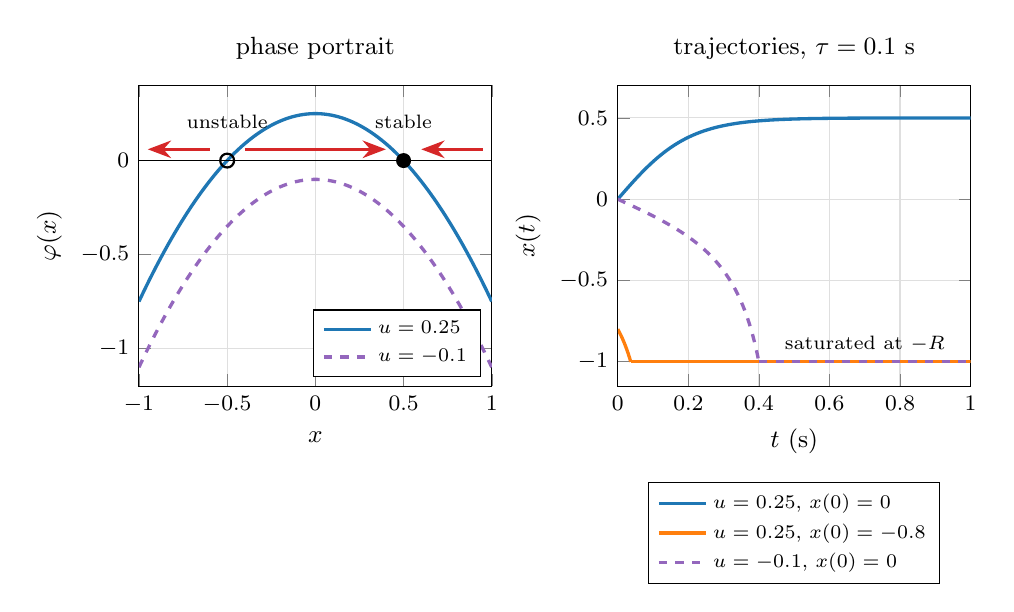
\begin{tikzpicture}
\begin{groupplot}[group style={group size=2 by 1, horizontal sep=1.6cm}, height=5.4cm]
\nextgroupplot[width=0.5\textwidth, xmin=-1, xmax=1, ymin=-1.2, ymax=0.4, xlabel={$x$}, ylabel={$\varphi(x)$},
  legend pos=south east, legend cell align=left, title={phase portrait}]
  \addplot[cA, very thick, domain=-1:1, samples=100] {0.25 - x^2};
  \addplot[cE, very thick, dashed, domain=-1:1, samples=100] {-0.1 - x^2};
  \legend{{$u = 0.25$}, {$u = -0.1$}}
  \addplot[black, thin, domain=-1:1, samples=2] {0};
  \addplot[only marks, mark=*, mark size=2.5pt, black] coordinates {(0.5,0)};
  \addplot[only marks, mark=o, mark size=2.5pt, black, thick] coordinates {(-0.5,0)};
  \draw[-{Stealth}, very thick, cD] (axis cs:-0.6,0.06) -- (axis cs:-0.95,0.06);
  \draw[-{Stealth}, very thick, cD] (axis cs:-0.4,0.06) -- (axis cs:0.4,0.06);
  \draw[-{Stealth}, very thick, cD] (axis cs:0.95,0.06) -- (axis cs:0.6,0.06);
  \node[font=\scriptsize, anchor=south] at (axis cs:0.5,0.12) {stable};
  \node[font=\scriptsize, anchor=south] at (axis cs:-0.5,0.12) {unstable};
\nextgroupplot[width=0.5\textwidth, xmin=0, xmax=1, ymin=-1.15, ymax=0.7, xlabel={$t$ (s)}, ylabel={$x(t)$},
  legend style={at={(0.5,-0.32)}, anchor=north}, legend cell align=left, legend columns=1, title={trajectories, $\tau = 0.1$ s}]
  \addplot[cA, very thick, domain=0:1, samples=100] {0.5*tanh(5*x)};
  \addplot[cB, very thick, domain=0:0.0368, samples=40] {0.5*cosh(5*x-0.733)/sinh(5*x-0.733)};
  \addplot[cE, very thick, dashed, domain=0:0.4, samples=80] {-sqrt(0.1)*tan(deg(sqrt(0.1)*x/0.1))};
  \draw[cB, very thick] (axis cs:0.0368,-1) -- (axis cs:1,-1);
  \draw[cE, very thick, dashed] (axis cs:0.4,-1) -- (axis cs:1,-1);
  \node[font=\scriptsize, anchor=south] at (axis cs:0.7,-1) {saturated at $-R$};
  \legend{{$u = 0.25$, $x(0) = 0$}, {$u = 0.25$, $x(0) = -0.8$}, {$u = -0.1$, $x(0) = 0$}}
\end{groupplot}
\end{tikzpicture}
\end{center}
\begin{marking}
0.5: parabola opening down, crossing at $\pm 0.5$, with arrows (right between the roots, left outside them). \ 0.5: $x(0) = 0$ goes to $+0.5$. \ 0.5: $x(0) = -0.8$ runs away to the negative saturation. \ 0.5: $u = -0.1$ has no equilibria and $x$ always decreases.
\end{marking}
\begin{trap}
Saying $x(0) = -0.8$ goes to $-0.5$. An unstable point repels, so a start beyond it moves \emph{away}.
\end{trap}

%=====================================================================
\section*{Question 4 \hfill (4)}

\ans{(a) [1]}
$A' = \tau A + I$ with $\tau\omega = 0.1 \cdot 2\pi = 0.2\pi \approx 0.63$:
\[
A' = \begin{bmatrix} 1 & -0.2\pi \\ 0.2\pi & 1\end{bmatrix} \approx \begin{bmatrix} 1 & -0.63 \\ 0.63 & 1\end{bmatrix}.
\]
\begin{marking}
0.5: identity on the diagonal. \ 0.5: off-diagonals $\mp\tau\omega = \mp 0.2\pi$ with the signs in the same places as $A$.
\end{marking}

\ans{(b) [2]}
Solve $\dot x_1 = -\omega x_2$ and $\dot x_2 = \omega x_1$ with $\mathbf x(0) = (0, 0.8)$:
\[
x_1(t) = -0.8\sin(2\pi t), \qquad x_2(t) = 0.8\cos(2\pi t).
\]
These are two sinusoids of amplitude $0.8$ and period $1$ s (two full cycles in $2$ s), $90^\circ$ apart. At $t = 0$, $x_2$ is at its peak and $x_1$ is heading \emph{negative}. In the plane, the state moves around a circle of radius $0.8$ \textbf{counter-clockwise}: from $(0, 0.8)$ to $(-0.8, 0)$ to $(0, -0.8)$ and back.
\begin{center}
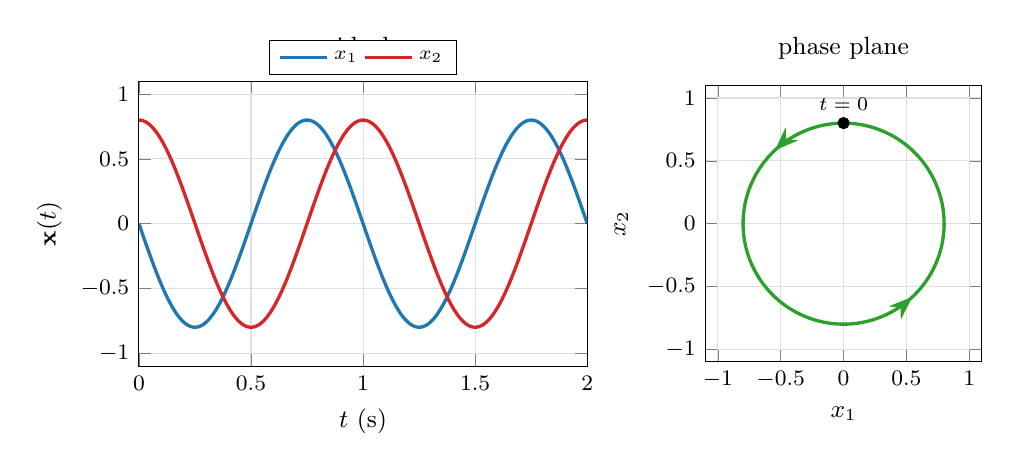
\begin{tikzpicture}
\begin{groupplot}[group style={group size=2 by 1, horizontal sep=1.5cm}, height=5.2cm]
\nextgroupplot[width=0.6\textwidth, xmin=0, xmax=2, ymin=-1.1, ymax=1.1, xlabel={$t$ (s)}, ylabel={$\mathbf x(t)$},
  legend style={at={(0.5,1.02)}, anchor=south}, legend cell align=left, legend columns=2, title={ideal}]
  \addplot[cA, very thick, domain=0:2, samples=200] {-0.8*sin(deg(2*pi*x))};
  \addplot[cD, very thick, domain=0:2, samples=200] {0.8*cos(deg(2*pi*x))};
  \legend{$x_1$, $x_2$}
\nextgroupplot[width=0.42\textwidth, xmin=-1.1, xmax=1.1, ymin=-1.1, ymax=1.1, axis equal image,
  xlabel={$x_1$}, ylabel={$x_2$}, title={phase plane}]
  \addplot[cC, very thick, domain=0:360, samples=120, postaction={decorate},
    decoration={markings, mark=at position 0.12 with {\arrow{Stealth[length=3mm]}}, mark=at position 0.62 with {\arrow{Stealth[length=3mm]}}}]
    ({-0.8*sin(x)}, {0.8*cos(x)});
  \addplot[only marks, mark=*, black] coordinates {(0,0.8)};
  \node[font=\scriptsize, anchor=south] at (axis cs:0,0.82) {$t = 0$};
\end{groupplot}
\end{tikzpicture}
\end{center}
\begin{marking}
0.5: both signals have period $1$ s and amplitude $0.8$. \ 0.5: $90^\circ$ apart with the right starting values ($x_1 = 0$, $x_2 = 0.8$). \ 0.5: circle of radius $0.8$. \ 0.5: counter-clockwise (from $(0, 0.8)$, $x_1$ goes negative first).
\end{marking}

\ans{(c) [1]}
\textbf{Kick:} $\mathbf x = 0$ is an equilibrium ($A'\mathbf 0 = \mathbf 0$). Without an input to move it off zero the network sits there forever. The kick sets the initial amplitude.

\textbf{Amplitude in Nengo:} ideally the circle keeps whatever amplitude the kick gave. In practice decoding errors make it slowly grow or shrink, and growth is capped by the \textbf{radius}: the neurons saturate, so the decoded value cannot go far past $|\mathbf x| \approx 1$. In the simulation below, a strong kick into $x_2$ makes the oscillator settle on a circle of radius about $0.9$.
\begin{center}
\begin{tikzpicture}
\begin{groupplot}[group style={group size=2 by 1, horizontal sep=1.5cm}, height=5cm]
\nextgroupplot[width=0.6\textwidth, xmin=0, xmax=3, ymin=-1.2, ymax=1.2, xlabel={$t$ (s)}, ylabel={decoded $\hat{\mathbf x}$},
  legend style={at={(0.5,1.02)}, anchor=south}, legend cell align=left, legend columns=2, title={Nengo, 800 LIF neurons, kick for $t < 50$ ms}]
  \addplot[cA, thick] table[x=t, y=x1] {pn3_data/q4_oscillator.dat};
  \addplot[cD, thick] table[x=t, y=x2] {pn3_data/q4_oscillator.dat};
  \legend{$\hat x_1$, $\hat x_2$}
\nextgroupplot[width=0.42\textwidth, xmin=-1.2, xmax=1.2, ymin=-1.2, ymax=1.2, axis equal image, xlabel={$\hat x_1$}, ylabel={$\hat x_2$}]
  \addplot[cC, thin] table[x=x1, y=x2] {pn3_data/q4_oscillator.dat};
  \addplot[gray, dashed, domain=0:360, samples=100] ({cos(x)}, {sin(x)});
\end{groupplot}
\end{tikzpicture}
\end{center}
\begin{marking}
0.5: zero is an equilibrium, so it needs a kick. \ 0.5: amplitude is set by the kick and limited by the radius or saturation (and decoding error).
\end{marking}

%=====================================================================
\section*{Question 5 \hfill (4)}

\ans{(a) [2]}
$x(t) = \int_0^t u\,dt'$:
\[
x(t) = \begin{cases} \int_0^t 4t'\,dt' = 2t^2, & 0 \le t < 0.5,\\ 2(0.5)^2 = 0.5, & t \ge 0.5.\end{cases}
\]
This is a parabola from $0$ to $0.5$, followed by a flat hold at $0.5$. The slope at $t = 0.5^-$ is $u = 2$, and it drops to $0$ instantly when the input stops, so the curve has a \emph{corner} at $t = 0.5$.
\begin{marking}
1: $2t^2$ on $[0, 0.5)$. \ 0.5: holds at $0.5$ after. \ 0.5: sketch is a parabola then flat (not a straight ramp).
\end{marking}

\ans{(b) [2]}
With different synapses on the input and the loop, $X = U/s + (\tau - \tin)\,U/(1 + s\tin)$. The decoded value is the true integral \textbf{plus an extra term $(\tau - \tin)$ times the (filtered) input}:
\[
\hat x(t) \approx 2t^2 + (0.1 - 0.01)\cdot 4t = 2t^2 + 0.36t \quad (t < 0.5).
\]
\begin{itemize}[leftmargin=1.2em]
\item The trace \textbf{runs ahead} of the ideal, and the gap grows with the input. Just before $t = 0.5$ s it is about $0.36 \times 0.5 \approx \mathbf{0.18}$, so $\hat x \approx 0.68$ instead of $0.5$ (the simulation gives about $0.63$--$0.65$, because the probe filter and decoding error shave a little off).
\item When the ramp stops, the extra term vanishes within a few $\tin$. The trace \textbf{drops back to $0.5$}, so the final value is still correct.
\end{itemize}
\begin{center}
\begin{tikzpicture}
\begin{groupplot}[group style={group size=1 by 2, vertical sep=0.4cm, xticklabels at=edge bottom}, width=0.95\textwidth, xmin=0, xmax=1]
\nextgroupplot[height=2.8cm, ymin=-0.2, ymax=2.3, ylabel={$u(t)$}]
  \addplot[black, very thick] table[x=t, y=u] {pn3_data/q5_ramp.dat};
\nextgroupplot[height=6cm, ymin=-0.05, ymax=0.8, xlabel={$t$ (s)}, ylabel={$x(t)$},
  legend style={at={(0.5,-0.3)}, anchor=north}, legend cell align=left, legend columns=2]
  \addplot[black, very thick, dashed] table[x=t, y=ideal] {pn3_data/q5_ramp.dat};
  \addplot[cB, very thick] table[x=t, y=lead] {pn3_data/q5_ramp.dat};
  \addplot[cA, thick] table[x=t, y=spike] {pn3_data/q5_ramp.dat};
  \addplot[cC, thick] table[x=t, y=rate] {pn3_data/q5_ramp.dat};
  \legend{{ideal (a): $2t^2$ then $0.5$}, {prediction: $\int u + (\tau - \tin)(h_{\mathrm{in}} * u)$}, {Nengo LIF, $\tin = 10$ ms}, {Nengo LIFRate, $\tin = 10$ ms}}
  \draw[{Stealth}-{Stealth}, cD, thick] (axis cs:0.49,0.48) -- (axis cs:0.49,0.66);
  \node[cD, font=\scriptsize, anchor=east] at (axis cs:0.48,0.6) {$\approx 0.36 \times 0.5 = 0.18$};
\end{groupplot}
\end{tikzpicture}
\end{center}
\begin{marking}
1: trace above the ideal during the ramp, with a gap that grows (proportional to $u$). \ 0.5: gap $\approx 0.18$ near $t = 0.5$ (accept $0.15$--$0.2$). \ 0.5: drops back to $0.5$ after the ramp stops (final value unchanged).
\end{marking}
\begin{trap}
Saying the faster input synapse only adds a small \emph{delay}. The mismatch adds an offset equal to $(\tau - \tin)u$, which is large here because $u$ reaches $2$.
\end{trap}

%=====================================================================
\section*{Bonus Question 1 \hfill (2)}
\textbf{Why it drifts:} an integrator holds its value only if the recurrent connection returns \emph{exactly} $x$, so that $\tau\dot x = f(x) - x = 0$ for every $x$. With a finite number of neurons the decoded $\hat f(x)$ is only approximately $x$. Wherever $\hat f(x) > x$ the value creeps up, and wherever $\hat f(x) < x$ it creeps down. The ``neural phase portrait'' $\hat f(x) - x$ is a small wiggly curve rather than zero. The state slides to the nearest point where that curve crosses zero going down, and stays there. These are the stable fixed points the decoding error creates by accident.

\textbf{Spiking vs rate:} in rate mode the decoding error is a fixed function of $x$, so the drift is deterministic and smooth (same network, same answer). With spikes, each neuron's output is a train of discrete pulses, so the fed-back signal also carries \textbf{spike noise}. The integrator integrates that noise too, which adds a random walk on top of the deterministic drift. Rate mode removes the noise only; the static distortion and its drift are still there.
\begin{marking}
1: drift comes from decoding (distortion) error, $\hat f(x) \neq x$, which creates fixed points the state slides toward. \ 1: spike noise is integrated (random walk); rate mode removes the noise but not the distortion.
\end{marking}

\end{document}
